\documentclass{article}

\usepackage[a4paper]{geometry}
\usepackage[ngerman]{babel}
\usepackage[utf8]{inputenc}
\usepackage[T1]{fontenc}
\usepackage{listings}
\usepackage{hyperref}
\usepackage{graphicx}
\usepackage{xcolor}
\usepackage{float}

\lstset{
    aboveskip=3mm,
    belowskip=3mm,
    showstringspaces=false,
    columns=flexible,
    basicstyle={\scriptsize\ttfamily},
    numbers=none,
    breaklines=true,
    breakatwhitespace=true,
    tabsize=4
}

\graphicspath{ {./images/} }

\hypersetup{colorlinks=true, allcolors=black}

\newcommand{\figuresource}[1]{
	\begin{center}Quelle: #1\end{center}
}

\title{Möglichkeiten zum Echtzeit-Video-Streaming im Web}

\author{
	\vspace{0.5em}
	Mara Schulke \textit{(Matrikel-Nr. 20215853)}\\
	\small{Technische Hochschule Brandenburg}\\
	\small{B.Sc. Medieninformatik}\\
	\small{Computergrafik}\\
	\small{Wintersemester 2021}\\
	\small{betreut durch Prof.\ Dr.\ rer.\ nat.\ Reiner Creutzburg}\\
}

\begin{document}

\begin{onecolumn}
	\begin{titlepage}
		\pagenumbering{gobble}


		\maketitle

		\begin{abstract}
			Durch die steigende dezentralisierung der Welt gewinnt die
			Echtzeit-Übertragung von Daten exponentiell an Relevanz. Die
			vorliegende Arbeit beschäftigt sich mit verschiedenen Protokollen
			zur Lösung dieses Problems und führt eine experimentelle
			Implementierung eines \textit{Peer-To-Peer} Kamera-Systems durch
			und wertet diese anschließend hinsichtlich der Qualität der
			Echtzeit-Übertragung, verbrauchten Ressourcen und ihres
			Implementierungsaufwandes aus.
		\end{abstract}

		\tableofcontents

		\listoffigures
	\end{titlepage}
\end{onecolumn}

\pagenumbering{arabic}

\begin{onecolumn}
\markboth{Hausarbeit Computergrafik – Mara Schulke}{}

\section{Einleitung / Motivation}

Mit der zunehmenden dezentralisierung und der damit einhergehenden Vernetzung
der Arbeitswelt in den letzten Jahren~\cite{CoronaHomeOffice} werden auch
digitale Meeting-Systeme immer relevanter und müssen immer mehr Nutzer in
Echtzeit mit einander verbinden um einen reibungslosen Arbeitsalltag zu
gewährleisten. Zu begin der Corona-Pandemie stieg der Netzwerktraffic für
\textit{Voice over IP} (kurz \textit{VoIP}) und Videokonferenzen im März 2020
um 210\%-285\%~\cite{NetzwerkStatistik}.

Damit die Konferenzsysteme ihren Einsatzzweck erfüllen können, ist es
erforderlich, dass eine ausreichend gute \textit{Quality of Service (QoS)}
gegeben ist.

Aber wie können skalierbare Meeting-Systeme realisiert werden ohne große
Datenmengen über einen zentralisierten Streaming-Server zu schicken der diese
an alle Teilnehmer weiterleitet? Die Entwicklungen der letzten Jahre deuten
immer mehr darauf hin, dass \textit{Peer-To-Peer} basierte Lösungensansätze
aufgrund der besseren Performance und Skalierbarkeit, in der Regel die bessere
Wahl darstellen~\cite{PeerToPeerVersusCentralized}.
\textit{Peer-To-Peer}-Architekturen halten einen unvorhersehbaren Anstieg in
der Nutzung deutlich besser aus, da die Echtzeit-Datenverarbeitung nicht bei
dem Konferenzsystem-Anbieter stattfindet, sondern bei den Teilnehmern.

Natürlich spielen zur Auswahl der Architektur noch weitere Parameter eine
wichtige Rolle (z. B. die maximale Bandbreite und Rechenleistung der
Endgeräte), aber mit immer größer werdenden Heimnetz-Leitungen und zunehmender
Rechenleistung der Endgeräte stellt dies mittlerweile für einfache
Videokonferenzen kein Problem mehr da.~\cite{VideokonferenzNetzwerklast}

Die Problematik der Echtzeit-Kommunikation im Web beschäftigt auch
das \textit{W3C} seit 2011 im Zuge der Standardisierung des seit diesem Jahr
zum Web-Standard erklärten Protokoll \textit{WebRTC}.~\cite{WebRTCStandardW3C}

Es ist also immer noch eine sehr aktuelle Thematik in der Informatik
Echtzeit- oder Nahe-Zu-Echtzeit-Kommunikation zuverlässig zu bewältigen.

Die Aufgabe dieser Arbeit soll sein, einen Überblick über den Stand der
Architekturmuster, Protokolle und möglicher Problematiken bei der
Implementierung von eigenen Echtzeit-Video-Streaming-Diensten geben. Dafür wird
im Rahmen eines Experiments ein Kamera-System implementiert. Die
Herangehensweise und Ansätze für die Implementierung werden erläutert und
anschließend wird das Ergebnis hinsichtlich der \textit{QoS} im Zusammenhang
mit dem Arbeitsaufwand ausgewertet.

\section{Historie der Echzeit-Übertragung}

Um zu verstehen wie sich die Protokolle hin zum heutigen Stand entwickelt
haben, ist es besonders interessant nachzuvollziehen wie die ersten Schritte
der IEFT oder auch \textit{Internet Engineering Task Force} bezüglich der
Echtzeit-Kommunikation aussahen, welche Probleme erkannt und behoben wurden und
welche Protokolle heute der Standard sind.

\subsection{1996: RTP \& RTCP}

Am weitesten reicht das \textit{Real-Time Transport Protocol} oder auch
\textit{RTP} zurück. Es wurde erstmals 1996 von der IEFT standardisiert und
stellt seit dem einen Grundbaustein der datenformatsaganostischen
Echtzeit-Übertragung da. Es kann für diverse
Echtzeit-Übertragungs-Problematiken dienlich sein, da jegliche Binärdaten
verschickt werden können; Somit gibt es keinen ``Lock-In'' auf bestimmte Audio-
oder Video-Codecs.

\textit{Realtime-Transport-Control-Protocol} oder auch \textit{RTCP} ist das
mit \textit{RTP} einhergehende Kontrollprotokoll. Es wird primär dazu
verwendet, die Übertragungsparameter der Sender zu beeinflussen – z. B. durch
ein Feedback zur Übertragungsqualität oder ein Abmelden der Session.
Desweiteren bietet es eine persistente ID für die \textit{RTP}-Mitglieder, die
über Programm-Neustarts hinweg zur Identifikation von Mitgliedern und der
zuordnung von Datenströmen verwendet werden können.~\cite{RFC1889}
% kapitel 6 / 6.1 bzw. S. 15-17

\textit{RTP und RTCP} siedeln sich im TCP/IP-Stack über \textit{UDP}
an.~\cite{RFC1889}

\textit{RTP} fügt wichtige Informationen zu UDP-Datagrammen hinzu: Im
wesentlichen eine Sequenznummer um die Sende-Reihenfolge zu codieren und einen
Payload-Type, der den Codec des Segments angibt. Somit kann auch bei nicht
sequenziell übertragenden Datagrammen die Ursprüngliche Reihenfolge
rekonstruiert werden und es können bei verlorenen Segmenten
Interpolationsalgorithmen verwendet werden. Der Payload-Type ist essenziell um
ohne Session-Aushandlung zu kommunizieren wie der Empfänger die Daten zu
decodieren hat, um eine sinnvolle Nachricht zu erhalten.

Die ersten Version aus 1996 wurde 2003 durch die überarbeitet Version,
spezifiziert in dem RFC3550, abgelöst.~\cite{RFC3550}

Eine wichtige Voraussetzung zur Verwendung von \textit{RTP} ist ein externer
\textit{Signaling-Server}, den alle Beteiligten zur Session-Aushandlung
verwenden. Ein Standard hierfür ist im \textit{RTP-Framework} selbst nicht
definiert, eine beliebte Wahl für ein Protokoll zur Session-Aushandlung ist
allerdings das \textit{Session Initiation Protokoll} oder kurz
\textit{SIP}.~\cite{RFC3550, RFC3261}

\subsection{2004:\ SRTP}

Im März 2004 wurden \textit{SRTP} und \textit{SRTCP} vorgestellt – die
verschlüsselten Version von \textit{RTP} bzw. \textit{RTCP}. Diese bauen
weitestgehend auf dem \textit{Advanced Encryption Standard} (kurz.
\textit{AES}) auf.~\cite{RFC3711} Der RFC beschäftigt sich weitestgehend mit
den kryptografischen Aspekten des Protokolls und ist in dieser Hinsicht für
dies vorliegende Arbeit nur bedingt interessant. Dennoch bildet
\textit{SRTP} eine wichtige Grundlage für sichere Echtzeitübertragung und
wird im WebRTC-Standard verwendet.

Eine weitverbreitete und offene Implementierung für \textit{SRTP / SRTCP}
wird von der US-Amerikanischen Telekomunikations-Gesellschaft Cisco
bereitgestellt. Diese hat den Namen \textit{libsrtp} und ist öffentlich auf der
Entwickler-Plattform GitHub öffentlich einsehbar (siehe
\url{https://github.com/cisco/libsrtp}).

% Anwendung in VoIP\!
% https://de.wikipedia.org/wiki/ZRTP

\subsection{2005: RTMP}

\textit{RTMP} ist ein von der Firma \textit{Adobe Systems Incorporated}
spezifiziertes Protokoll zur Echtzeit-Übertragung von Multimedia-Streams.
\textit{RTMP} wurde laut Spezifikation~\cite{RTMPSpec} entwickelt um
über dem Transport-Protokoll \textit{TCP} verwendet zu werden.

Das Protokoll wurde dazu entwickelt um im Kontext eines Flash-Players verwendet
zu werden. Dies führt dazu, dass es heutzutage nurnoch bedingt in Browsern
Anwendung findet, da mittlerweile viele Browser ihren Flash-Player-Support
eingestellt haben.~\cite{RTMPFlashSupport}

Außerdem spricht die hohe Latenz von bis zu 30 Sekunden, die durch die
Verwendung von \textit{TCP} zustandekommt~\cite{StreamingProtokolle} gegen den
Einsatz von \textit{RTMP} in einem Echtzeit-Übertragungs-Kontext.

Desweiteren gibt nach~\cite{RTMP} noch weitere Protokollvarianten:

\begin{itemize}
	\item \textit{RTMPT} (Tunneled) verwendet \textit{HTTP} bzw. \textit{HTTPS}
		als Transport-Protokoll.
	\item \textit{RTMPE} (Encrypted)
	\item \textit{RTMPTE} (Tunneled und Encrypted)
	\item \textit{RTMPS} verwendet \textit{SSL}
	\item \textit{RTMFP} verwendet \textit{UDP} als Transport-Protokoll
		anstelle von \textit{TCP}
\end{itemize}

Auch wenn \textit{RTMP} aufgrund der hohen Latenz für Videokonferenzen
ungeeignet ist, findet es heutzutage immernoch Anwendungen in
unidirektionalen Datenübertragungen an eine große Anzahl von Teilnehmern, da es
sich gut skalieren lässt.~\cite{RTMP}

\subsection{2006: DTLS}

Das \textit{Datagram-Transport-Layer-Security}-Protokoll bietet starke
Sicherheitsgarantien (equivalent zu \textit{TLS}) für Datagram basierte
Protokolle wie z. B. \textit{UDP}.~\cite{RFC4347} Es bildet heutzutage die
Grundlage für sichere, verbindungslose Kommunikation.

\subsection{2010: WebRTC}

\textit{WebRTC} ist eine Peer-To-Peer-Technologie die über mehrere Protokolle
und Audio- und Video-Codecs performante und generische
Echtzeit-Kommunikations-Kanäle zwischen Nutzern (oder auch \textit{Peers})
realisiert. Dafür stellt eine \textit{WebRTC}-Implementierung durch einen
komplexen Signaling-Ablauf eine direkte Verbindung zu anderen Endgeräten
her.~\cite{MDNSignaling}

\subsubsection{Signaling}

Während der Signaling-Phase generiert zunächst einer der Teilnehmer eine
\textit{SDP-Offer}. Diese wird über einen, nicht näher im Standard
beschreibenen, Signaling-Channel an den anderen Teilnehmer gesendet.
Dieser verarbeitet die \textit{SDP-Offer} und generiert eine
\textit{SDP-Answer} und sendet diese über den gleichen Signaling-Channel an den
Absender zurück.

Nach erfolgreichem austauschen der \textit{SDP}-Nachrichten,
verwendet generiert jeder Teilnehmer mithilfe des \textit{Interactive
Connectivity Establishment}-Frameworks \textit{ICE}-Candidates und versendet
sie über den Signaling-Channel. Diese werden verwendet um einen eindeutigen
Weg durch das Internet zum anderen Teilnehmer zu finden. Dieser Vorgang ist
notwendig, da durch die Einführung \textit{Network-Address-Translation}, in den
meisten Netzwerken Endgeräte keine globale eindeutige IPv4-Adresse
haben.~\cite{MDNSessionLifetime}

\subsubsection{Übertragung}

Sobald die Signaling-Phase erfolgreich beendet wurde und beide Teilnehmer sich
im Internet gefunden haben, wird eine direkte \textit{SRTP}-Verbindung
hergestellt.~\cite{RFC8834} Diese wird über \textit{DTLS}
verschlüsselt.~\cite{RFC8827}

Anschließend können die zu übertragenden Daten in den entsprechenden Codecs
über diese Verbindung versendet werden.

\section{Architekturmuster}

In diesem Kapitel werden zwei der bekanntesten Architekturmuster in der
Echtzeit-Übertragung vorgestellt und verglichen. Es geht primär um die
verteilte Peer-To-Peer Architektur und die zentralisierte Relay / Broadcast
Architektur.

\subsection{Peer-To-Peer}

Auf Grund der hohen Anforderungen an möglichst niedrige Übertragungslatenzen
bietet eine Peer-To-Peer-Architektur klare Vorteile durch den stark verkürzten
Weg, den die Pakete zurücklegen müssen bis sie bei dem Empfänger ankommen.

Deutlich komplizierter wird allerdings die aushandlung bzw.\ initialisierung
einer Verbindung zwischen zwei peers, da diese sich nicht wie bei der typischen
Client-Server-Architektur eine fixe adresse zur verbindung haben. Dieses
Problem wird typischerweise über einen Signaling-Server gelöst.

\subsubsection{Signaling-Server}
Ein Signaling-Server ist allen Teilnehmern bekannt und dient als
Kommunikationsplattform. Somit können sich zwei, sich initial unbekannte
Teilnehmer, gegenseitig vorstellen.

Signaling-Server sind interessanterweise keine feste Anforderung für
Peer-To-Peer-Architekturen. Wenn alle Teilnehmer statische Addressen hätten,
könnten sie auch Out-Of-Band ihre IP-Adressen und ggf.\ weitere Details zum
Verbindungsaufbau austauschen, um eine Verbindung aufzubauen.

Der Signaling-Server kann weiterhin noch nach Verbindungsaufbau dazu verwendet
werden um die bestehende Verbindung zu optimieren. Peers können neue
ICE-Candidates vorschlagen um die Übertragung an neue Gegebenheiten anzupassen.

\subsubsection{Theoretische Optimierung durch IP-Multicast}

Je mehr Nutzer / Endgeräte an einer Peer-To-Peer-Übertragung teilnehmen, desto
größer wird die Belastung der Bandbreite bei den einzelnen Teilnehmern. Jedes
Paket muss nicht einmal, sondern $N$-mal verschickt werden (wobei $N$ die
Anzahl der Teilnehmer ist). Dies kann bei labilen oder einfach schwachen
Netzwerken entweder zur Verminderung der Übertragungsqualität führen, oder in
besonders schlimmen Fällen sogar das restliche Netzwerk eines einzelnen
Teilnehmers negativ beeinflussen, da dieser die meiste Bandbreite für die
wiederholte Übertragung gleicher Pakete verwendet.

Eine theoretische Lösung für dieses Problem, ist die Verwendung von
IP-Multicast-Adressen. Diese erlauben es einem Gerät ein IP-Paket einmalig zu
übertragen, und dieses von Multicast-Routern im Internet multiplizieren zu
lassen.

Dieser Ansatz hat klare Vorteile: Das gesamte - lokale \& globale – Netzwerk
wird geschont. So würde die Anzahl möglicher Teilnehmer deutlich steigen, da
ein Netzwerk-Bottleneck erst bei einem zu großen Download-Volumen des
empfangenen Contents eintreten würde.

Leider ist dies aus verschiedenen Gründen bisher nur in der Theorie möglich.
Der Hauptgrund ist die mangelnde Unterstützung für IPv4-Multicast-Pakete bei
einem Großteil der Router. Desweiteren würden Heimnetzwerke somit in
Backbonenetzwerken deutlich mehr Netzwerklast auslösen können als vorgesehen
ist.

\subsection{Relay}

Die zentralisierte Architektur ist eine der besten Alternativen zum
Peer-To-Peer-Ansatz. Sie wird bei diversen Streaming-Plattformen erfolgreich
bei einer großen Anzahl von Nutzern betrieben.~\cite{YoutubeRTMP, TwitchRTMP}
Der wohl grundlegenste Unterschied liegt darin, dass zwischen den Teilnehmern
eine zentralisierte Instanz geschaltet ist, die den Stream vervielfacht um so
die Netzwerkauslastung bei einzelnen Teilnehmern zu minimieren.

Diese Architektur lässt im Gegensatz zu Peer-To-Peer-Architekturen deutlich
mehr Teilnehmer zu, da nur der Relay-Server die Last skalieren muss und nicht
ein Teilnehmer. Wenn ein Live-Stream auf einer Streaming-Plattform
beispielsweise einige Hundert Zuschauer hat und dies via Peer-To-Peer laufen
würde, wäre dies bereits eine Größe bei der typische Endgeräte und
Heimnetzwerke definitiv überlastet wären.

Folglich finden zentralisierte Architekturen auch bei Mobilgeräte
anwendung~\cite{YoutubeRTMP, TwitchRTMP}, da Mobilgeräte oft (abgesehen von
einer stärker limiterten Bandbreite) lediglich über ein fixes Datenvolumen
verfügen.

Zu den Vorteilen zählt die einfache Skalierbarkeit, die (weitestgehende)
Unabhängigkeit von Teilnehmer Netzwerken und die Kontrolle über den verteilten
Datenstrom.

Die Nachteile hingegen zeichnen sich für die Teilnehmer in einer erhöhten
Latenz ab, was ein Relay für Live-Videokonferenzen in der Regel uninteressanter
macht. Desweiteren fallen Hosting-Kosten in direkter Abhängig von der
Nutzeranzahl ab, da jeder Datenstrom vom Server verarbeitet wird.

\section{Implementierung eines Kamera-Live-Streams}

In diesem Kapitel wird ein experimentelles Kamera-System entwickelt. Dieses
baut auf einem WebSocket-Secure basierten Signaling-Protokoll, \textit{WebRTC}
und \textit{GStreamer} auf.

\subsection{Ziel}

Ziel dieses Experiments ist es eine möglichst einfach ein funktionierendes
Kamera-System zu entwickeln und mögliche Probleme, benötigten Zeitaufwand etc.\
zu ermitteln. Zukünftig könnte noch ein Performance-Vergleich mit anderen
Echtzeit-Systemen interessant sein.

Es gilt also die Frage zu klären, wie viel Arbeit ein simples, aber
funktionierendes Software-Produkt das auf Echtzeit-Übertragung beruht benötigt
und wie gut die Übertragungsqualität anschließend ist.

\subsection{Umfang}

Das zu implementierende Kamera-System wird lediglich eine einzige
Kernfunktion aufweisen: Sobald die Kamera an ist, streamt sie via
WebRTC, mit ausreichend FPS (mindestens 15 im durchschnitt) in
ausreichender Qualität (720$\times$480), ihre Aufnahmen an eine
Benutzeroberfläche. Diese wird im Browser laufen, muss aber ausreichend
Alternativen für andere Plattformen aufweisen (Nativ, Smartphone
usw.). Die Benutzeroberfläche und die Kamera starten die Aushandlung des
WebRTC-Streams über den Signaling-Server. D.h.\ sie versenden
\textit{SDP}-Nachrichten und tauschen ihre \textit{ICE}-Candidates aus
(siehe~\figurename~\ref{fig:signaling}).

\subsection{Architektur}

\begin{figure}[ht]
	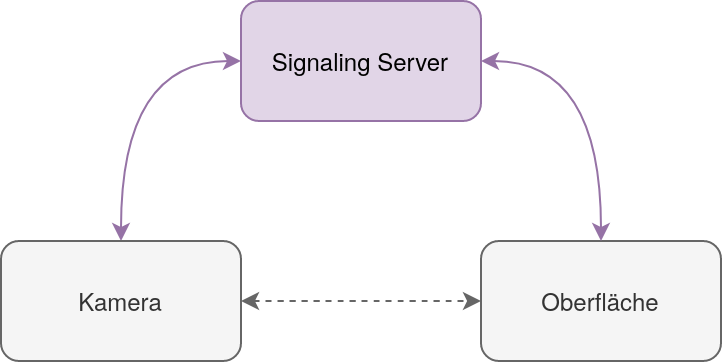
\includegraphics[width=0.5\textwidth]{diagram-signaling}
	\centering
	\caption{Signaling zwischen der Kamera und der Benutzeroberfläche.}\label{fig:signaling}
	\figuresource{Schulke 2021, nach~\cite{WebRTC}}
\end{figure}

Die geplante Architektur ist besteht lediglich aus 3 Elementen:

\subsubsection{Kamera}

Für dieses Experiment wurde ein Einplatinencomputer der Marke Raspberry PI in
der 4. Version mit 8GB RAM – erweitert durch ein Drittanbieter-Kamera-Modul –
verwendet. Dieser ist allerdings absolut austauschbar, da jeder Rechner der
die u.g. Hauptanforderung erfüllt eine geeignete Umgebung darstellt – so kann
die Kamera-Software auch auf einem Laptop ausgeführt werden, falls keine
Hardware verfügbar ist. Dies wurde zur veranschaulichung mit einem ThinkPad
T490 und einer aktuellen NixOS Installation getestet.

Die Hauptanforderung an die Hardware auf der die Kamera-Software läuft ist eine
Linux-Installation (mit den entsprechenden installierten Paketen für die
Abhangigkeiten) und eine angeschlossene Kamera die von Linux erkannt wird.

Auf der Einplatinencomputer ist das mitgelieferte Betriebssystem ``Raspberry PI
OS'' und die entsprechenden Software-Abhängigkeiten (siehe~\ref{items:deps})
installiert.

\subsubsection{Signaling-Server}

Der Signaling-Server ist ein WebSocket-Secure-Server, der zwei
WebSocket-Verbindungen miteinander verknüpft. Er verwaltet sogenannte Räume.
Ein Raum besteht aus 0 bis 2 Teilnehmer und dient dazu diese miteinander zu
verbinden. Auf dem Server kann es mehrere Räume gleichzeitig geben – dadurch
könnte dieser Signaling-Server theoretisch auch noch für weitere
WebRTC-Anwendungen verwendet werden. Ein Raum hat eine ID, diese ist eine
256-Bit-Entropie. Teilnehmer werden durch eine 128-Bit-Entropie identifiziert.

So können sich zwei Teilnehmer durch ein Out-Of-Band kommuniziertes Secret (die
Raum-ID) über diesen in Kontakt treten. Diese könnte beispielsweise, würde es
sich bei der entwickelten Kamera um ein echtes Produkt handeln, bei der
Herstellung generiert werden, ausgedruckt und neben die Kamera in die
Verpackung gelegt werden.

\subsubsection{Benutzeroberfläche}

Die Benutzeroberfläche verbindet sich mit dem Signaling-Server und nimmt eine
Raum-ID entgegen. Mit dieser Raum-ID wird dann auf dem Signaling-Server
entweder ein neuer Raum erstellt, falls noch keiner mit der ID existiert, oder
es wird dem bestehenden Raum beigetreten. Nach dem ein weiterer Teilnehmer
beigetreten ist, fängt der unter~\ref{sec:signaling-spec} erklärte Aufbau eines
WebRTC-Streams zu dem Nutzer an.

\subsection{Signaling-Server}

Als erstes wurde der Signaling-Server entwickelt, da dieser keine
Abhängigkeiten an seine Teilnehmer hat. Die Kamera-Software und
Benutzeroberfläche setzen beide jeweils den laufenden Signaling-Server vorraus
um korrekt zu funktioneren.

\subsubsection*{Asynchronität}

Eine logische Anforderungen an den Server ist das gleichzeitige verarbeiten
mehrerer Verbindungen – ansonsten könnte immer nur ein Teilnehmer alleine mit
dem Server Verbunden sein. Dies würde die Signaling-Funktionalität eines Raumes
unbrauchbar machen.

Die asynchrone Programmierung ist ein Konzept zur Lösung dieser Problemklasse.
Da langlebige Verbindungen in der Regel einen großteil der Zeit ungenutzt sind,
ist es naheliegend Verbindungen ohne neue Ereignisse keine CPU-Zeit zu geben
um andere Verbindungen in der Zeit abzuarbeiten, in der auf Ereignisse gewartet
wird.

\subsubsection{Verbindungsaufbau}

Um eine WebSocket-Secure-Verbindung aufzubauen, muss zu erst eine TCP- und dann
darüber eine TLS-Verbindung zu dem Teilnehmer aufgebaut werden. Über diese wird
dann zu erst in HTTP kommuniziert und nach einer erfolgreichen Nachricht des
Servers mit dem Status-Code 101 (Switching Protocols) wird die über den
gleichen Transport-Weg (TLS) nach dem WebSocket-Protokoll kommuniziert.

\subsubsection{Spezifikation des Signaling-Protokolls}\label{sec:signaling-spec}

Das Signaling-Protokoll ist in 2 Nachrichten-Typen unterteilt:
Server-Nachrichten und Peer-Nachrichten. Teilnehmer dürfen nur Peer-Nachrichten
senden, ansonsten wird die Verbindung aufgrund eines Protokoll-Verstoßes
geschlossen. Der Server verschickt nur Server-Nachrichten.

Alle Protokoll-Nachrichten werden in JSON kodiert und dann über den
WebSocket-Nachrichten-Typ Binär an den Empfänger geschickt werden.

\vspace{0.5em}

\textbf{Server-Nachrichten}

\begin{itemize}
	\item Hello \{Teilnehmer-ID\}
	\item Joined
	\item Error
	\item Room/Join \{Teilnehmer-ID\}
	\item Room/Leave \{Teilnehmer-ID\}
	\item Room/Signal \{Signal\}
\end{itemize}

\vspace{0.5em}

\textbf{Peer-Nachrichten}

\begin{itemize}
	\item JoinOrCreate \{Raum-ID\}
	\item Signal \{Signal\}
\end{itemize}

\vspace{0.5em}

Nach einer erfolgreich aufgebauten Verbindung mit dem Server schickt dieser ein
\textit{Hello} mit der zugewiesenen Teilnehmer-ID.\ Darauf hin muss der
Teilnehmer ein \textit{JoinOrCreate} senden um einem Raum beizutreten. Bevor
der Teilnehmer die Nachricht \textit{Joined} vom Server erhält, darf dieser keine
Signale verschicken.

Eine \textit{Room/Join} Nachricht wird an ggf.\ andere Teilnehmer im Raum
verschickt, sobald ein Teilnehmer diesen betritt. Diese Nachricht kann auf dem
Teilnehmer als Anlass genutzt werden eine SDP-Offer zu erstellen, da nun sicher
ist, das ein anderer Teilnehmer im Raum ist. Wenn beide Teilnehmer sich an dieses
Schema halten, schickt immer der Teilnehmer, der sich zu erst Verbunden hat die
Einladung und der andere die Answer.

Analog wird eine \textit{Room/Leave} Nachricht verschickt wenn ein Teilnehmer
einen Raum verlässt.

Die \textit{Room/Signal} Nachricht wird an den Empfänger eines Signals
geschickt, nachdem der Sender des Signals eine \textit{Signal} Nachricht an den
Server geschickt hat.

Siehe \figurename~\ref{fig:signaling-protocol-flow} für einen kompletten
WebRTC-Verbindungsaufbau.

\begin{figure}[ht]
	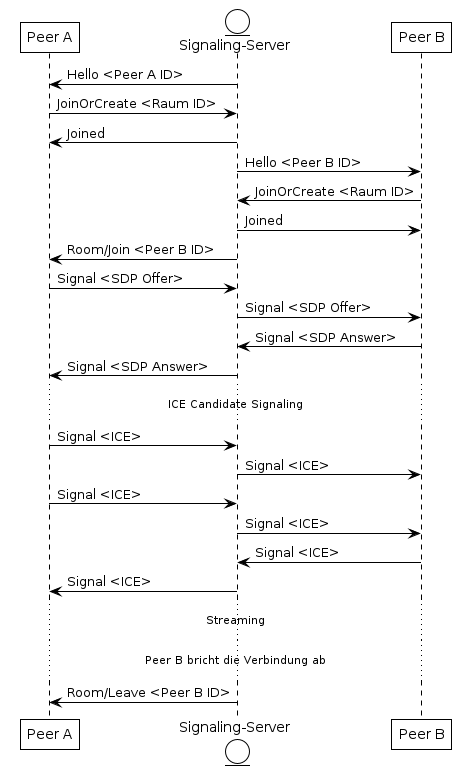
\includegraphics[width=0.5\textwidth]{signaling-protocol}
	\centering
	\caption{Anwendungsbeispiel des Singaling-Protokolls}\label{fig:signaling-protocol-flow}
	\figuresource{Schulke 2021}
\end{figure}

\subsubsection{Raum-Verwaltung}

Die Raum-Verwaltung fällt unter anderem in die Kategorie der
Synchronisationsprobleme. Es gibt unter Umständen $n$ Teilnehmer-Verbindungen,
die den Status von einem Raum erfragen wollen, und ggf.\ einen Anlegen möchten.
Dies soll für alle Verbindungen öffentlich geschehen, Teilnehmer dürfen sich
aber dabei nicht gegenseitig überschreiben.

Um zwei asynchron laufende Programmteile zum sequenziellen Zugriff auf
gemeinsamen Speicher zu zwingen, gibt es Möglichkeit einen Semaphor bzw. Mutex
zu verwenden. Dieser blockiert den Teil des Programms, der gerade auf den
gemeinsamen Speicher zugreifen möchte solange, bis ein ggf.\ anderer Zugriff
beendet ist. Um Deadlocks bzw. Inperformante Code-Abschnitte zu vermeiden, ist
es ratsam einen Mutex nicht über länger andauernde Operationen hinweg zu
locken, da sonst für diese Zeit alle anderen Teile des Programms, die gerade
auf den Speicher zugreifen möchten blockiert sind.

Als konkrete Lösung für das bestehende Problem bietet sich eine HashMap, deren
zugriff von einem Mutex kontrolliert wird, an. Jede Teilnehmer-Verbindung, die
aktuelle Raum-Informationen braucht (was hauptsächlich bei dem erstellen /
betreten von Räumen der Fall ist), muss nun vorher erst den mutex locken. 

\subsubsection{Kommunikation zwischen mehreren Teilnehmer-Verbindungen}

Bis zu diesem Punkt ist der Aufbau der Verbindung und das zu implementierende
Protokoll klar, allerdings fehlt noch das Verknüpfen von
Teilnehmer-Verbindungen um Signale weiterzuleiten.

Da bereits Räume verwaltet werden, liegt es nahe dort einen Kommunikationskanal
einzubetten. Eine Implementierung für diesen Kommunikationskanal stellen z.B.
sogenannte Channels dar. Diese erlauben Inter-Thread- (und im asynchronen
Kontext: Inter-Task-) Kommunikation über ein einfaches
Sender-Empfänger-Prinzip. Ein Channel ist unterteilt in eben diese beiden
Teile: Der Sender darf Nachrichten schreiben, der Empfänger darf sie aus dem
Channel lesen.

In diesem Fall ist allerdings zusätzlich noch bidirektionale Kommunikation
gefragt, da beide Teilnehmer die Signale des jeweils anderen erhalten sollen.
Dafür bieten sich sogenannte Broadcast-Channel an. Sie sind dafür ausgelegt,
dass von mehreren Stellen in diese geschrieben und gelesen wird. Sie
funktioneren analog zu dem Broadcast aus der Netzwerktechnik (siehe
\figurename~\ref{fig:broadcast}).

\begin{figure}[ht]
	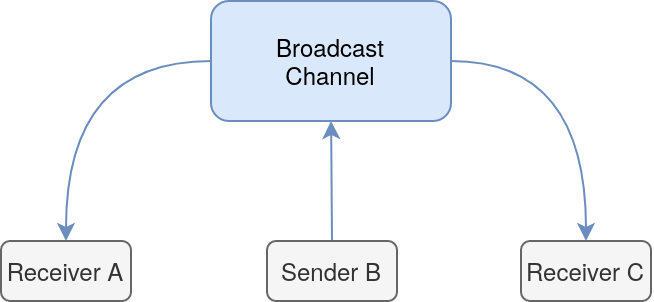
\includegraphics[width=0.5\textwidth]{diagram-broadcast}
	\centering
	\caption{Broadcast-Channel Konzept}\label{fig:broadcast-channel}
	\figuresource{Schulke 2021}
\end{figure}

Somit kriegt jeder Teilnehmer bei betreten eines Raumes Zugriff auf einen
Sender und einen Empfänger dieses Broadcast-Channels. In diesen schreibt er bei
erhalt einer Peer-Nachricht vom Typ \textit{Signal} das Signal (siehe
\figurename~\ref{fig:broadcast-usage}). Eine Teilnehmer-Verbindung die gerade
keine CPU-Zeit erhält, da ansonsten keine Ereignisse aufgetreten sind, wird
wieder aktiv sobald eine neue Nachricht über den Channel da ist.  Diese kann
dann als Server-Nachricht vom Typ \textit{Room/Signal} mit dem Signal aus dem
Channel an den Empfänger gesendet werden.

\begin{figure}[ht!]
	\includegraphics[width=0.5\textwidth]{diagram-websocket-verknüpfung}
	\centering
	\caption{Kommunikation von Nutzern über einen Broadcast-Channel}\label{fig:broadcast-usage}
	\figuresource{Schulke 2021}
\end{figure}

\subsection{Benutzeroberfläche}

Um den Signaling-Server für ein erstes nutzbares Zwischenergebnis zu verwenden,
wurde eine einfache browserbasierte Benutzeroberfläche implementiert, die
analog zu sehr bekannten Videokonferenz-Systemen wie z.B. Zoom oder Google Meet
funktioniert. Bei diesem Experiment wurde der Fokus primär auf die
Bildübertragung gelegt – eine Audioübertragung könnte aber ohne großen Aufwand
implementiert werden.

Ein Benutzer muss über diese Benutzeroberfläche einem beliebigen Raum auf dem
Signaling-Server beitreten können. Sobald ein weiterer Benutzer beitritt soll
der erste eine Nachricht erhalten, dass Jemand seinem Raum beigetreten ist.
Letztendlich soll die Aushandlung der Video-Übertragung zwischen den beiden
Benutzern ohne weitere Interaktion des Benutzers stattfinden.

\subsubsection{WebSocket-Verbindung}

Als Vorkehrungen für die singalisierungs Kommunikation mit dem Signaling-Server
muss eine WebSocket-Secure Verbindung mit dem Server aufgebaut werden. Dies
gelingt ebenfalls über eine Web-API.\

Nun meldet sich der Server nach dem Verbindungsaufbau als erstes mit der
\textit{Hello}-Nachricht und weist uns eine ID zu. Nach dieser ersten Nachricht
können wir die eigentliche Anwendung starten.

\subsubsection{Erstellen / Beitritt eines Raumes}

Um festzustellen mit wem sich der Benutzer verbinden möchte, muss dieser
eine Raum-Id angeben. Diese ist als 64 Zeichen langen Hex-String einzugeben.

Nach erfolgreicher Eingabe einer Raum-Id wird diese mit der Nachricht
\textit{JoinOrCreate} an den Server geschickt, dieser verarbeitet die Anfrage
und schickt dem Benutzer eine \textit{Joined}-Nachricht. Ab diesem Zeitpunkt
wird eine \textit{RTCPeerConnection} erstellt, da ggf.\ bereits ein anderer
Nutzer im Raum war, der dem neu dazugekommenen eine SDP-Offer schicken wird.
Um diese Zeitnah zu verarbeiten, findet die Initialisierung vor der ersten
Signalisierungs-Nachricht statt.

\subsubsection{Verbindungsaufbau}\label{browser-webrtc}

Moderne Browser wie Firefox, Chrome, Safari etc.\ stellen eine Implementierung
des WebRTC-Standards bereit (siehe \figurename~\ref{fig:webrtc-support}), die
durch eine übersichtliche API leicht zu integrieren ist.

\begin{figure}[ht]
	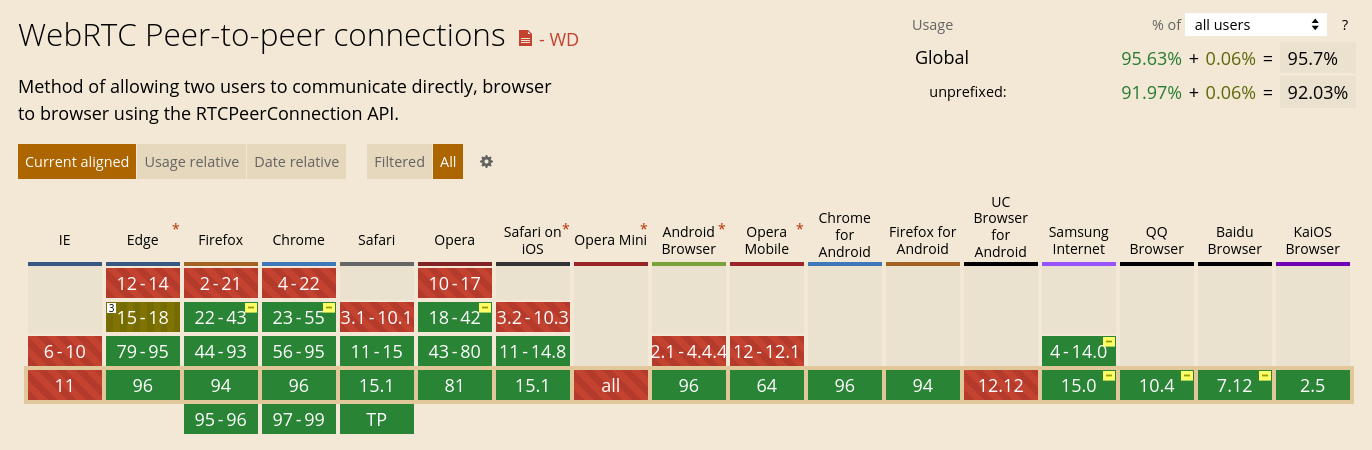
\includegraphics[width=0.5\textwidth]{webrtc-support}
	\centering
	\caption[WebRTC Support-Matrix~\cite{WebRTCSupport}]{WebRTC Support-Matrix}\label{fig:webrtc-support}
	\figuresource{\cite{WebRTCSupport}}
\end{figure}

Um eine vollständige WebRTC-Verbindung aufzubauen ist bei beiden Nutzern eine
RTCPeerConnection aufzubauen. Auf einer RTCPeerConnection ist eine
Event-basierte API verfügbar. (Siehe tabelle)

% table mit der API und der quelle der API:

Insbesondere sind für den Verbindungsaufbau die Events onnegotiationneeded und
onicecandidate von Interesse. Sobald eine Verbindung erstellt wurde und ein
lokaler Stream zu dieser hinzugefügt wurde, wird das onnegotiationneeded Event
ausgelöst. An diesem Punkt ist nun eine eigene SDP-Offer zu erstellen und über
den singalisierungs Server an den Empfänger zu versenden. Der Empfänger
verarbeitet diese anschließend und antwortet mit einer SDP-Answer. Nach dem
beide Teilnehmer die SDP-Nachrichten füe ihren Kommunikationspartner und sich
selbst gesetzt haben (siehe setRemoteDescription und setLocalDescription),
werden vom Browser onicecandidate-Events ausgelöst um eine direkte Verbindung
zwischen den beiden Browsern auszuhandeln.

% Signalisierungsablauf zwischen Benutzeroberflächen und Kamera visualisiert:

\begin{figure}[ht]
	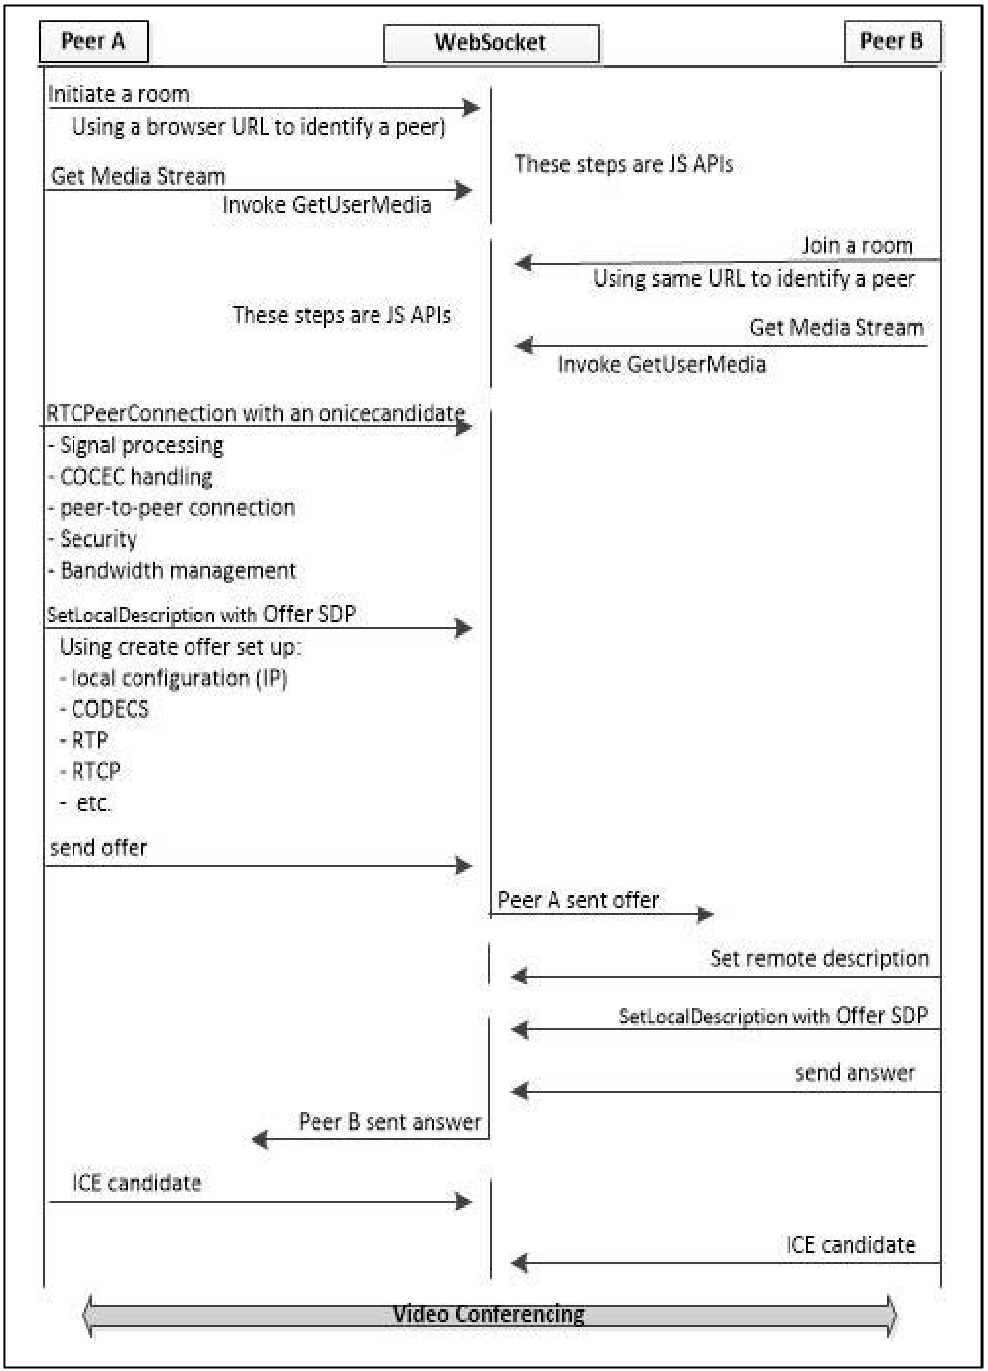
\includegraphics[width=0.5\textwidth]{cited-webrtc-connection-establishment}
	\centering
	\caption[WebRTC-Verbindungsaufbau~\cite{WebRTC}]{WebRTC-Verbindungsaufbau}
	\figuresource{\cite{WebRTC}}
\end{figure}

Nach einem leeren ICE-Kandidaten ist die aushandlung abgeschlossen und der
Stream kann nun konsumiert werden.

\subsubsection{Verbindungsabbau}

Nach dem der Signalisierungs-Server eine \textit{Room/Leave}-Nachricht gesendet
hat, kann die RTCPeerConnection ohne negative Auswirkungen abgebaut werden. In
der Benutzeroberfläche wird die Anzeige des Video-Streams des anderen
Teilnehmers zurückgesetzt und die RTCPeerConnection geschlossen. Somit ist die
Benutzeroberfläche wieder bereit einem weiteren Raum beizutreten und erneut
eine WebRTC Verbindung herzustellen.

% Screenshots der Demo Benutzeroberfläche anfügen

\subsection{Kamera}

\subsubsection{GStreamer}

Anders als in einer Browser-Umgebung bietet Linux abgesehen von der
bereitstellung von Hardware-Treibern keine guten Abstraktionen für die
Verwendung einer Kamera und automatischer Bildverarbeitung. Dies ist in einer
nativen Umgebung die Aufgabe von weiteren Programmen und Bibliotheken.

Hier wird das weitverbreitete Multimedia-Framework GStreamer relevant. Dieses
abstrahiert sämtliche Zugriffe auf medienbezogene Hardware (in diesem Fall die
Kamera), beherscht die meistgenutzten Media-Codecs für Audio und Video und kann
über Plugins mit weiteren Funktionalitäten erweitert werden (siehe
\figurename~\ref{fig:gstreamer-arch}).

GStreamer ist dafür ausgelegt das erstellen von Audio und/oder Video basierten
Anwendung zu erleichtern. Es unterstützt weiterhin, durch die
Pipeline-Architektur, jegliche Art von Datenströmen.

% Siehe https://gstreamer.freedesktop.org/documentation/application-development/introduction/gstreamer.html?
% Siehe https://gstreamer.freedesktop.org/documentation/application-development/introduction/gstreamer.html?

\begin{figure}[ht]
	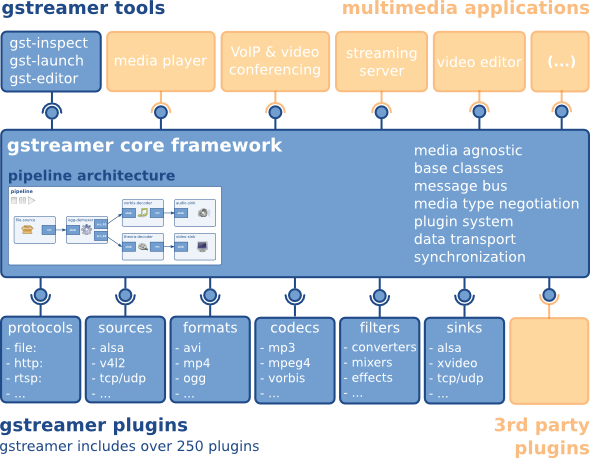
\includegraphics[width=0.5\textwidth]{gstreamer-overview.png}
	\centering
	\caption[GStreamer Architektur~\cite{GStreamerManualIntro}]{GStreamer Architektur}\label{fig:gstreamer-arch}
	\figuresource{\cite{GStreamerManualIntro}}
\end{figure}

Zu den Kern-Features von GStreamer gehören eine API für diverse
Multimedia-Anwendungen, eine Pipeline- und Plugin-Architektur, Mechanismen für
die Aushandlung von Datenformaten zwischen Pipeline-Elementen, Synchronisation
von Datenströmen. (siehe \figurename~\ref{fig:gstreamer-arch},~\cite{GStreamerManualIntro})

Das Framework baut auf einem ausgereiften Plugin-System mit über 250 Plugins
auf, welches den Codec-Support erweitert und weitere Komponenten zur Erstellung
von komplexeren Pipelines bereitstellt.

Diese Plugins können in die folgenden Kategorien unterteilt werden:

\begin{itemize}
	\item Protokolle
	\item Datenquellen
	\item Formate
	\item Codecs
	\item Filter \& Effekte
	\item Ausgabe
\end{itemize}

Siehe~\cite{GStreamerManualIntro}\\

Für dieses Experiment ist das GStreamer-Plugin für WebRTC besonders von
bedeutung.

Somit muss die folgende Liste an Abhängigkeiten installiert werden, damit die
Kamera-Software korrekt funktioniert:

\begin{itemize}\label{items:deps}
	\item libgstreamer-gl1.0-0
	\item libgstreamer-opencv1.0-0
	\item libgstreamer-plugins-bad1.0-0
	\item libgstreamer-plugins-base1.0-0
	\item libgstreamer1.0-0
	\item libgstrtspserver-1.0-0
\end{itemize}

\subsubsection{Architektur der Kamera-Software}

Die Kamera-Software ist grundsätzlich in 2 Zustände unterteilt, die sich endlos
abwechseln:

\begin{enumerate}
	\item Verbindungsaufbau zum Signalisierungsserver
	\item Streaming via WebRTC
\end{enumerate}

Im Regelfall dauert der 1. Schritt einige Millisekunden. Nach dem die
Verbindung zum Signalisierungsserver korrekt aufgebaut wurde (und die Kamera
dem festgelegten Raum beitreten konnte) wird eine GStreamer-Pipeline
initialisiert und auf den Beitritt eines Benutzers in den Raum erwartet. Nach
dem die \textit{Room/Join}-Nachricht eingetroffen wird die Pipeline auf Playing
gesetzt.

GStreamer unterstützt nach erfolgreicher Installation oben genannter Plugins
eine kompatible API zu der der Browser. Somit läuft der gesamte
WebRTC-Spezifische Verbindungsaufbau nach der exakt gleichen Logik ab wie
unter\ \ref{browser-webrtc} erläutert.

Bei der Einbindung von \textit{GStreamer} wurde~\cite{GStreamerExamples} als
Referenz verwendet.

\subsubsection{Vorbereitung der Laufzeitumgebung}

Sobald die Kamera-Software auf einem herkömlichen Desktop-System lauffähig ist,
gilt es die Laufzeitumgebung auf der Kamera-Hardware vorzubereiten.

Hierfür muss zunächst das Betriebssystem der Hardware, Raspberry PI OS,
installiert werden. Anschließend sind die unter~\ref{items:deps} aufgezählten
Software-Abhängigkeiten zu installieren. Sobald diese vorhanden sind, kann die
Kamera-Software auf anderen Desktop-Systemen für die entsprechende
System-Architektur (\textit{armv7-unknown-linux-gnueabihf}) kompiliert werden
und anschließend auf den Einplatinencomputer übertragen werden.

\subsubsection{Automatischer Start der Kamera-Software}

Da die Kamera-Hardware nicht permanent Stromzufuhr haben wird, ist es hilfreich
einen Betriebssystem-Service für anzulegen, der für die automatische Ausführung
der Software verantwortlich ist. Somit muss nicht bei jedem Neustart händisch
die Software ausgeführt werden.

Unter Raspberry PI OS übernimmt diese aufgabe der Init-Service Systemd.

% \section{Benchmarks}
% - CPU Load
% - Netzwerkauslastung
% - Zeitaufwand für Impl

\section{Auswertung}

Der Signaling-Server hatte den größten Implementierungsaufwand der 3
Komponenten, hat sich dafür aber als sehr stabil und vielseitig einsetzbar
erwiesen. Hinsichtlich der Performance ist die Implementierung ebenfalls ein
Erfolg. Auf einem System mit einem Intel i7-8565U-Chip übersteigt der Server
mit 50 Benutzern nicht annähernd 1\% der CPU-Kapazität. Falls nicht eine
große Anzahl an Nutzern gleichzeitig viele Signale über diesen Server schickt,
pendelt sich dieser aufgrund seiner asynchronen Architektur bei einer
CPU-Last von 0.0\% ein, da dieser nur aktiv wird, wenn auch Nachrichten
eintreffen.

Die Benutzeroberfläche ist rein funktional geblieben und bietet kein gutes
Nutzererlebnis. Abgesehen von der schlechten Nutzbarkeit, ist die erwartete
Funktionalität vollständig und mit angemessenem Aufwand implementierbar
gewesen. Die Browser-APIs bieten eine exzellente Grundlage um reale
Anwendungen in kurzer Zeit mit einer Live-Stream-Funktionalität zu entwickeln.
Desweiteren funtkioniert auch die Videoübertragung vom Browser über eine
WebRTC-Verbindung sehr gut, die Bildübertragungsraten waren in der
Regel über den angestrebten 15 Bildern pro Sekunde.

Die Implementierung einer Kamera-Software ist im Vergleich zu den beiden
anderen Komponenten verhältnismäßig aufwändig gewesen. GStreamer bringt
ebenfalls vergleichbare WebRTC-Abstraktionen mit sich, wie moderne Browser,
allerdings ist GStreamer erheblich instabiler und unzuverlässiger was den
Stream-Aufbau angeht als die Browser. Auch die Bildübertragungsrate ist leider
erst bei sehr niedriger Qualität (160px$\times$90px) nah an dem angestrebten
Wert. Sobald die Qualität diese überschritt, nimmt die Bildübertragungsrate
drastisch ab und somit wird der Stream ab einer gewissen Bildqualität
unbrauchbar. Dies könnte ggf.\ auf das 32-Bit-Betriebssystem der Hardware
zurückzuführen zu sein.

\section{Nächste Schritte}

Einer der nächsten Schritte um dieses Experiment weiterzuführen wäre definitiv
die Fehlersuche an der Kamera-Software um die Übertragungsqualität zu steigern.

Außerdem sollte die Kamera-Software nicht erneut dem Raum auf dem
Signaling-Server beitreten sobald der Stream abbricht, dies zu beheben könnte
eine (auch wenn nur geringe) Netzwerkentlastung bringen und würde zusätzlich
den Signaling-Server schonen.

Auch die Sicherheit von Räumen könnte durch ausgreiftere
Authentifizierungsverfahren drastisch erhöht werden.

Als letzte Verbesserung wäre eine Implementierung von Audio-Übertragung von der
Kamera zu der Benutzeroberfläche interessant um auch diesen Aspekt der
Echtzeitübertragung im Web auszustesten.

% Mögliche Optimierungen:
% - Verbesserung der Video-Qualität: Evtl kein 32bit os
% - Nicht ständig signalisieren, einmal joinen als kamera
% - Kamera interface verbessern
% \large{IPV6 only => NAT holepunching entfällt}

\nocite{*}

\bibliographystyle{IEEEtran}
\bibliography{IEEEabrv, references}

\end{onecolumn}

\begin{onecolumn}
\begin{appendix}

\section*{Anhang}

\begin{scriptsize}
	\begin{flushleft}
		\texttt{\textbf{signaling/main.rs}}
		%\lstinputlisting{implementation/signaling/src/main.rs}
		\texttt{\textbf{signaling/lib.rs}}
		%\lstinputlisting{implementation/signaling/src/lib.rs}
		\texttt{\textbf{signaling/tls.rs}}
		%\lstinputlisting{implementation/signaling/src/tls.rs}
		\texttt{\textbf{signaling/rooms.rs}}
		%\lstinputlisting{implementation/signaling/src/rooms.rs}
		\texttt{\textbf{signaling/state.rs}}
		%\lstinputlisting{implementation/signaling/src/state.rs}
		\texttt{\textbf{signaling/signals.rs}}
		%\lstinputlisting{implementation/signaling/src/signals.rs}
		\texttt{\textbf{camera/main.rs}}
		%\lstinputlisting{implementation/camera/src/main.rs}
		\texttt{\textbf{camera/webrtc.rs}}
		%\lstinputlisting{implementation/camera/src/webrtc.rs}
		\texttt{\textbf{camera/signaling.rs}}
		%\lstinputlisting{implementation/camera/src/signaling.rs}
		\texttt{\textbf{interface/index.html}}
		%\lstinputlisting{implementation/interface/index.html}
	\end{flushleft}
\end{scriptsize}

\begin{figure*}[p]
	%\includegraphics[width=0.5\textwidth]{photo-board}
	\centering
	\caption{Rapsberry PI 4}
\end{figure*}

\begin{figure*}[p]
	%\includegraphics[width=0.5\textwidth]{photo-cam}
	\centering
	\caption{Camera Modul}
\end{figure*}

\begin{figure*}[p]
	%\includegraphics[width=0.5\textwidth]{photo-installed}
	\centering
	\caption{Installierte Kamera}
\end{figure*}

\end{appendix}
\end{onecolumn}

% TODO: Jede Abbildung erwähnen
% TODO: Jede Section auf Rechtschreibung prüfen
% TODO: Zitate checken!
% TODO: Fehlende Tabellen einbauen
% TODO: Centricular zitieren

\end{document}
